\documentclass[a4paper, 12pt]{article}

\usepackage{tikz}
\usetikzlibrary{automata, positioning, arrows}
\usepackage{float}
\usepackage[left=2cm, right=2cm, top=2cm, bottom=2cm]{geometry}

\tikzset{
	->,
	node distance=3cm, 
	>=stealth',
	every state/.style={thick},
	baseline}

\begin{document}
\pagenumbering{roman}
\title{
		\textbf{Group Members}\\ 
		Tevin Achong - 816000026\\
		Jimmel Greer - 816000045\\
		\textbf{Course Code:} COMP3602\\
		\textbf{Course Title:} Theory of Computing\\
		\textbf{Assignment:} 1
		\date{October 24, 2019}
}
\maketitle

\newpage
\begin{enumerate}

\item %1
\begin{itemize}
\item[(a)] $\{0^n \lor 1^m$ $|$ $n$ is even, $m$ is odd$\}$ ~\\

\begin{figure}[H]
	\centering
	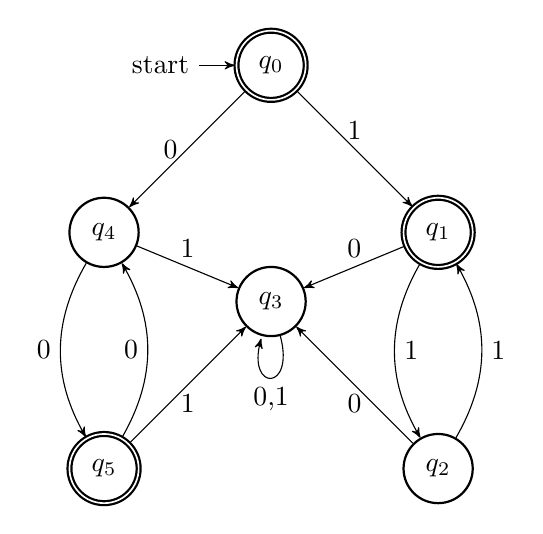
\begin{tikzpicture}
		
		\node[state, initial, accepting] (q0) {$q_0$};
		\node[state, accepting, below right of=q0] (q1) {$q_1$};
		\node[state, below of=q1] (q2) {$q_2$};
		\node[state, below of=q0] (q3) {$q_3$};
		\node[state, below left of=q0] (q4) {$q_4$};
		\node[state, accepting, below of=q4] (q5) {$q_5$};
		
		\draw 
		(q0) edge[above] node{1} (q1)
		(q0) edge[left] node{0} (q4)
		(q1) edge[bend right, right] node{1} (q2)
		(q1) edge[above] node{0} (q3)
		(q2) edge[bend right, right] node{1} (q1)
		(q2) edge[below] node{0} (q3)		
		(q3) edge[loop below, below] node{0,1} (q3)
		(q4) edge[above] node{1} (q3)
		(q4) edge[bend right, left] node{0} (q5)
		(q5) edge[bend right, left] node{0} (q4)
		(q5) edge[below] node{1} (q3)
		;
			
		
	\end{tikzpicture}
\end{figure}

\item[(b)] Any string that does not contain the substring 01 ~\\

\begin{figure}[H]
	\centering
	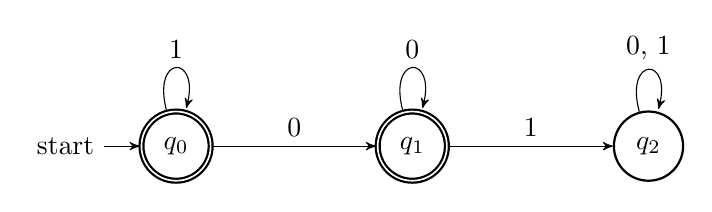
\begin{tikzpicture}
	
		\node[state, initial, accepting] (q0) {$q_0$};
		\node[state, accepting, right of=q0] (q1) {$q_1$};		 	
		\node[state, right of=q1] (q2) {$q_2$};
		
		\draw
		(q0) edge[loop above, above] node{1} (q1)
		(q0) edge[above] node{0} (q1)
		(q1) edge[loop above, above] node{0} (q1)
		(q1) edge[above] node{1} (q2)
		(q2) edge[loop above, above] node{0, 1} (q2)
		;
	
	\end{tikzpicture}
\end{figure}
\end{itemize}

\newpage
\item %2
\begin{itemize}
\item[(a)] Strings ending in 1011 ~\\

\begin{figure}[H]
	\centering
	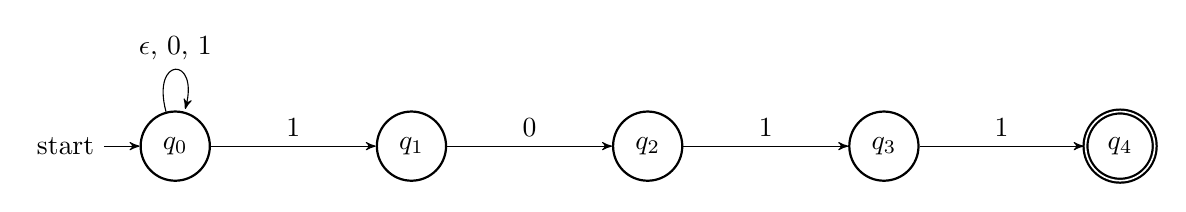
\begin{tikzpicture}
		\node[state, initial] (q0) {$q_0$};
		\node[state, right of=q0] (q1) {$q_1$};
		\node[state, right of=q1] (q2) {$q_2$};
		\node[state, right of=q2] (q3) {$q_3$};
		\node[state, accepting, right of=q3] (q4) {$q_4$};
		
		\draw
		(q0) edge[above] node{1} (q1)
		(q0) edge[loop above, above] node{$\epsilon$, 0, 1} (q1)
		(q1) edge[above] node{0} (q2)
		(q2) edge[above] node{1} (q3)
		(q3) edge[above] node{1} (q4)
		;
	\end{tikzpicture}
\end{figure}

\item[(b)] $\{101x101$ $|$ $x \in \Sigma^*\}$ ~\\
\begin{figure}[H]
	\centering
	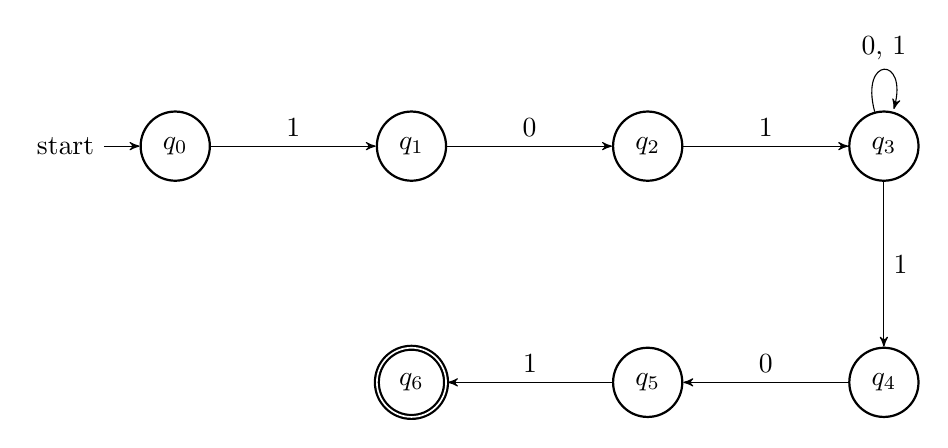
\begin{tikzpicture}
		\node[state, initial] (q0) {$q_0$};
		\node[state, right of=q0] (q1) {$q_1$};
		\node[state, right of=q1] (q2) {$q_2$};
		\node[state, right of=q2] (q3) {$q_3$};
		\node[state, below of=q3] (q4) {$q_4$};
		\node[state, left of=q4] (q5) {$q_5$};
		\node[state, accepting, left of=q5] (q6) {$q_6$};
		
		\draw
		(q0) edge[above] node{1} (q1)
		(q1) edge[above] node{0} (q2)
		(q2) edge[above] node{1} (q3)
		(q3) edge[right] node{1} (q4)
		(q3) edge[loop above, above] node{0, 1} (q3)
		(q4) edge[above] node{0} (q5)
		(q5) edge[above] node{1} (q6)
		;
	\end{tikzpicture}
\end{figure}

\end{itemize}

\newpage
\item %3
Let us refer to the DFA in Question 1b as $M$. Then 
$ M = \{\{q_0, q_1, q_2\}, \{0, 1\}, \delta, q_0, \{q_0, q_1\}\} $
where $ \delta $ is given by:\\
$\delta(q_0, 0) = q_1$\\
$\delta(q_0, 1) = q_0$\\
$\delta(q_1, 0) = q_1$\\
$\delta(q_1, 1) = q_2$\\
$\delta(q_2, 0) = q_2$\\
$\delta(q_2, 1) = q_2$\\
 
\item %4
Let us refer to the NFA in Question 2b as $N$. Then 
$ N = \{\{q_0, q_1, q_2, q_3, q_4, q_5, q_6\}, \{0, 1\}, \delta, q_0, \{q_6\}\} $
where $ \delta $ is given by:\\
$\delta(q_0, 0) = \{\}$\\
$\delta(q_0, 1) = \{q_1\}$\\
$\delta(q_0, \epsilon) = \{\}$\\
$\delta(q_1, 0) = \{q_2\}$\\
$\delta(q_1, 1) = \{\}$\\
$\delta(q_1, \epsilon) = \{\}$\\
$\delta(q_2, 0) = \{\}$\\
$\delta(q_2, 1) = \{q_3\}$\\
$\delta(q_2, \epsilon) = \{\}$\\
$\delta(q_3, 0) = \{q_3\}$\\
$\delta(q_3, 1) = \{q_3, q_4\}$\\
$\delta(q_3, \epsilon) = \{\}$\\
$\delta(q_4, 0) = \{q_5\}$\\
$\delta(q_4, 1) = \{\}$\\
$\delta(q_4, \epsilon) = \{\}$\\
$\delta(q_5, 0) = \{\}$\\
$\delta(q_5, 1) = \{q_6\}$\\
$\delta(q_5, \epsilon) = \{\}$\\
$\delta(q_6, 0) = \{\}$\\
$\delta(q_6, 1) = \{\}$\\
$\delta(q_6, \epsilon) = \{\}$\\

\newpage
\item %5 

\item %6

\item %7

\item %8

\item ~\\%9
\begin{center}
	\begin{tabular}{|c|c|c|}
	\hline
	\textbf{Regular Expression} & \textbf{Recognized Strings} & \textbf{Non-Recognized Strings}\\
	\hline
	$a^*b^*$ & &\\
	\cline{2-3}
	& &\\
	\hline
	$a(ba)^*bb$ & &\\
	\cline{2-3}
	& &\\
	\hline
	$a^+ \cup b^*$ & &\\
	\cline{2-3}
	& &\\
	\hline
	$(\epsilon \cup a)b$ & &\\
	\cline{2-3}
	& &\\
	\hline
	\end{tabular}
\end{center}
\end{enumerate}


\pagenumbering{arabic}
\end{document}